\documentclass[
	aspectratio=169, % default is 43
	8pt, % font size, default is 11pt
	handout, % handout mode without animations, comment out to add animations
]{beamer}
\def\university{}

\documentclass[
	aspectratio=169, % default is 43
	8pt, % font size, default is 11pt
	handout, % handout mode without animations, comment out to add animations
]{beamer}

\usepackage{../template/beamerthemeuulm} % use the inofficial uulm beamer theme
\setfaculty{infIngPsy} % set the color scheme for your faculty here [med/infIngPsy/math/nat]

% requires symbolic links
% git clone git@github.com:SoftVarE-Group/SlideTemplate.git C:\Users\...\SlideTemplate
% mklink /J template C:\Users\...\SlideTemplate
% git clone git@spgit.informatik.uni-ulm.de:thuem/slides.git C:\Users\...\ThomasSlides
% mklink /J thomasslides C:\Users\...\ThomasSlides
\graphicspath{{../template/pics/logos}{../template/pics/nature}{../template/pics/uulm}{../thomasslides/}{../pics/people/}{../pics/xkcd/}}

%\usepackage[ngerman]{babel} % use this line for slides in German
%\recordingtrue % special recording mode for use with a greenscreen, gives you space to show yourself in a layer in front of the slides, has no effect in the handout mode

\title{Software Product Lines} % short title is used for the slide footer but optional

% LINKED LITERATURE

\newcommand{\ludewiglichter}{\href{https://learning.oreilly.com/library/view/-/9781457184932/?ar}{Ludewig and Lichter}}
\newcommand{\seeconomics}{\href{https://rds-ulm.ibs-bw.de/link?kid=027381854}{SE Economics}}
\newcommand{\sommervillelink}[1]{\href{https://ulm.ibs-bw.de/aDISWeb/app?service=direct/0/Home/$DirectLink\&sp=SOPAC00\&sp=SAKSWB-IdNr1615420983}{#1}}
\newcommand{\sommerville}{\sommervillelink{Sommerville}}
\newcommand{\thehumbleprogrammer}{\href{https://dl.acm.org/doi/10.1145/1283920.1283927}{The Humble Programmer}}
\newcommand{\thepragmaticprogrammer}{\href{https://learning.oreilly.com/library/view/the-pragmatic-programmer/9780135956977/}{The Pragmatic Programmer}}

% TYPICAL COMMANDS FOR LECTURES

\renewcommand{\emph}[1]{{\color{blue}\textbf{#1}}}

\newcommand{\deutsch}[1]{{\color{blue}(#1)}}
\newcommand{\deutschertitel}[1]{{\tiny\deutsch{#1}}}

\newcommand{\mycite}[1]{``#1''}
\newcommand{\mytitlesource}[1]{{\tiny\normalfont\mbox{[#1]}}}
\newcommand{\mysource}[1]{\ifthenelse{\equal{#1}{}}{}{\phantom{.}~\hfill~\mytitlesource{#1}}}

\newcommand{\todo}[1]{{\color{red}\textbf{[#1]}}}
\newcommand{\fodo}[1]{\todo{\footnote{\todo{#1}}}}
\newcommand{\todots}{\todo{\ldots}}

% IMPORTED PACKAGES

%\usepackage{adjustbox} % used for partofpage
%\usepackage{tcolorbox} % used for mydefinition, mynote, myexample
\usepackage{multicol} % used temporarily for the lecture overview
\usepackage{mathtools} % required for absolute value in modeling lecture

% COMMANDS TO LAYOUT AND ANNIMATE SLIDES

\newcommand{\lessonslearned}[3]{
	\subsection{Summary}
	\begin{frame}{\insertsection -- \insertsubsection}
		\leftorright{
			\mydefinition{Lessons Learned}{
				\begin{itemize}
					#1
				\end{itemize}
			}
			\mynote{Further Reading}{
				\small % references take space, can be a little smaller
				\begin{itemize}
					#2
				\end{itemize}
			}
		}{
			\myexample{Practice}{
				#3
			}
		}
	\end{frame}
}

% TODO temporary hack to layout the slide overview in two colums
\renewcommand{\lectureoverview}{
%	\section*{Overview}
%	\subsection*{Overview}
	\begin{frame}{\insertsubtitle}
		\begin{multicols}{2}
			\tableofcontents
		\end{multicols}
	\end{frame}
}

\renewcommandx{\maketitle}[2][1=apr21-o25a,2=150]{
    {
	\usebackgroundtemplate{} % TODO temporary hack to enable missing pictures at title slide
	%\ifx {#1} \empty \else {\usebackgroundtemplate{\includegraphics[trim=0 0 0 #2,clip,width=\paperwidth]{#1}}} \fi     
	%\usebackgroundtemplate{\includegraphics[trim=0 0 0 #2,clip,width=\paperwidth]{#1}}
    \begin{frame}[plain]
        \vskip0pt plus 1filll
        \begin{beamercolorbox}[wd=\paperwidth,ht=4.5ex,dp=2ex,right]{titlebox}
            \LARGE\textbf{\inserttitle}\hspace*{20pt}
        \end{beamercolorbox}%
        \nointerlineskip%
        \begin{beamercolorbox}[wd=\paperwidth,ht=2.25ex,dp=1ex,right]{subtitlebox}
            \small 
            \ifx \insertsubtitle \empty \else \insertsubtitle\ $\vert$ \fi
            \insertauthor\
            \ifx \insertdate \empty \else $\vert$ \insertdate \fi
            \hspace*{20pt}
        \end{beamercolorbox}%
        \nointerlineskip%
        \begin{beamercolorbox}[wd=\paperwidth,ht=4.5ex,dp=2ex,left]{logobox}
            \centering
            \vspace{-1ex}
            \hspace{10pt}
            \includegraphics[height=4.5ex]{sp} % SPECIFY INSTITUTE LOGO HERE
            \hfill
            \includegraphics[height=4.5ex]{uulm}
            \hspace{10pt}
        \end{beamercolorbox}%
    \end{frame}
    }  
}

%
%\newcommand{\onlyleft}[1]{
%	\halfpage{#1}
%}
%
%\newcommand{\onlyright}[1]{
%	~\hfill
%	\halfpage{#1}
%}
%
%\newcommand{\leftorright}[2]{
%	\uncover<1>{\halfpage{#1}}
%	\hfill
%	\uncover<3->{\halfpage{#2}}
%}
%
%\newcommand{\rightorleft}[2]{
%	\uncover<3->{\halfpage{#1}}
%	\hfill
%	\uncover<1>{\halfpage{#2}}
%}
%
%\newcommand{\leftthenright}[2]{
%	\halfpage{#1}
%	\hfill\pause
%	\halfpage{#2}
%}
%
%\newcommand{\leftandright}[2]{
%	\halfpage{#1}
%	\hfill
%	\halfpage{#2}
%}
%
%\newcommand{\leftmiddleandright}[3]{
%	\thirdpage{#1}
%	\hfill
%	\thirdpage{#2}
%	\hfill
%	\thirdpage{#3}
%}
%
%\newcommand{\leftmiddleorright}[3]{
%	\uncover<1>{\thirdpage{#1}}
%	\hfill
%	\uncover<3>{\thirdpage{#2}}
%	\hfill
%	\uncover<5->{\thirdpage{#3}}
%}
%
%\newcommand{\halfpage}[1]{\partofpage{48}{#1}}
%
%\newcommand{\thirdpage}[1]{\partofpage{31}{#1}}
%
%\newcommand{\partofpage}[2]{
%	\adjustbox{valign=t}{\begin{minipage}{0.#1\textwidth}
%			\begin{flushleft}
%				#2
%			\end{flushleft}
%	\end{minipage}}
%}
%
%\newcommand{\mydefinition}[2]{
%	\begin{tcolorbox}[title=#1,colback=orange!10,colframe=orange!30,coltitle=black,fonttitle=\bfseries,left=1mm,right=1mm,top=1mm,bottom=1mm]
%		\begin{flushleft}
%			#2
%		\end{flushleft}
%	\end{tcolorbox}
%}
%
%\newcommand{\mydefinitiontight}[2]{
%	\begin{tcolorbox}[title=#1,colback=white,colframe=orange!30,coltitle=black,fonttitle=\bfseries,left=0mm,right=0mm,top=0mm,bottom=0mm]
%		\begin{flushleft}
%			#2
%		\end{flushleft}
%	\end{tcolorbox}
%}
%
%\newcommand{\mynote}[2]{
%	\begin{tcolorbox}[title=#1,colback=red!10,colframe=red!30,coltitle=black,fonttitle=\bfseries,left=1mm,right=1mm,top=1mm,bottom=1mm]
%		\begin{flushleft}
%			#2
%		\end{flushleft}
%	\end{tcolorbox}
%}
%
%\newcommand{\myexample}[2]{
%	\begin{tcolorbox}[title=#1,colback=blue!10,colframe=blue!30,coltitle=black,fonttitle=\bfseries,left=1mm,right=1mm,top=1mm,bottom=1mm]
%		\begin{flushleft}
%			#2
%		\end{flushleft}
%	\end{tcolorbox}
%}
%
%\newcommand{\myexampletight}[2]{
%	\begin{tcolorbox}[title=#1,colback=white,colframe=blue!30,coltitle=black,fonttitle=\bfseries,left=0mm,right=0mm,top=0mm,bottom=0mm]
%		\begin{flushleft}
%			#2
%		\end{flushleft}
%	\end{tcolorbox}
%}

\subtitle{3. Compile-Time Variability with Clone-and-Own}
\author{Timo Kehrer, Thomas Thüm, Elias Kuiter}
\foruniversity{}
	{\setpicture[70]{ovgu-autumn2}\setcopyright{Photo: Hannah Theile (OVGU)}}
	{\setpicture{oct20-south4}}

\begin{document}

\mode<handout>{\contentoverview}

\mode<beamer>{
	\ifdefined\thepicture
		\maketitle[\thepicture][\thepictureoffset]
	\else
		\maketitle[]
	\fi
}

% shared slide content

% introduced: 02a-configuration
% reused: 03a-intro
\newcommand{\frameImplementSPLs}{
	\begin{mycolumns}[widths={45},animation=none]
		\pic[width=\linewidth]{metaproduct2}
	\mynextcolumn
		\begin{note}{Key Issues}
			\begin{itemize}
			\item Systematic reuse of implementation artifacts
			\item Explicit handling of variability
			\end{itemize}
		\end{note}
		\uncover<2->{\begin{definition}{Variability\mysource{\fospl\mypage{48}}}
			\mycite{\emph{Variability} is the ability to derive different products from a common set of artifacts.}
		\end{definition}}
		~
		\uncover<3->{\begin{note}{Variability-Intensive System}
			Any software product line is a variability-intensive system. % TODO Timo: do we really need this term? where does this definition come from?
		\end{note}}
	\end{mycolumns}
}

% introduced: 02a-configuration
% reused: 02b-implementation, 03a-intro
\newcommand{\frameVariabilityAndBindingTimes}{
	\begin{mycolumns}[widths={55},animation=none]
		\begin{definition}{Binding Time \deutsch{Bindungszeitpunkt}\mysource{\fospl\mypage{48}}}
			\begin{itemize}
				\item Variability offers choices
				\item Derivation of a product requires to make decisions (aka. binding)
				\item Decisions may be bound at different binding times
			\end{itemize}
		\end{definition}
		~
		\uncover<2->{\begin{note}{When? By whom? How?}
			\lectureruntime\parta: \emph{when} and \emph{by whom}

			\lectureruntime\partb: \emph{how}
		\end{note}}
	\mynextcolumn
		\pic[width=\linewidth]{metaproduct2}
	\end{mycolumns}
}

% introduced: 03a-intro
% reused: 03a-intro
\newcommand{\frameRuntimeVariabilityProblems}{
	\begin{note}{Problems of Runtime Variability}
		{\bf Conditional Statements:}
		\begin{itemize}
			\item Code scattering, tangling, and replication
		\end{itemize}
		{\bf Design Patterns for Variability:}
		\begin{itemize}
			\item Trade-offs and potential negative side effects
			\item Constraints that may restrict their usage
		\end{itemize}
		{\bf In General:}
		\begin{itemize}
			\item Variable parts are always delivered
			\item Not well-suited for compile-time binding
		\end{itemize}
	\end{note}
}

% introduced: 03a-intro
% reused: 03a-intro
\newcommand{\frameSoftwareConfigurationManagement}{
	\begin{mycolumns}
		\begin{definition}{Software Configuration Management} % TODO source missing
			Policies, processes, and tools for managing evolving software systems:
			\begin{itemize}
				\item Version control
				\item System building
				\item Release management
				\item Change management
				\item Collaborative work
			\end{itemize}
		\end{definition}
	\mynextcolumn
		\begin{note}{No Software Configuration Management}
			\lecturecloneandown\parta: Ad-Hoc Clone-and-Own

			aka.\ unmanaged clone-and-own
		\end{note}
		\begin{note}{Version Control}
			\lecturecloneandown\partb: Clone-and-Own with Version Control

			instance of managed clone-and-own
		\end{note}
		\begin{note}{System Building}
			\lecturecloneandown\partc: Clone-and-Own with Build Systems

			instance of managed clone-and-own
		\end{note}
	\end{mycolumns}
}


\section{Compile-Time Variability and Clone-and-Own}

\subsection{Recap: Runtime Variability}
\begin{frame}{\insertsubsection}
	\leftorright{
		Basic principles
		\mynote{Runtime parameters}{
			\begin{itemize}
				\item Conditional statements controlled by configuration parameters
				\item Global variables vs. method parameter passing
			\end{itemize}	
		}
		\mynote{Object-oriented concepts and Design Patterns}{
			\begin{itemize}
				\item Template Method
				\item Abstract Factory
				\item Decorator
				\item etc.
			\end{itemize}	
		}
	}{
Problems

Configuration parameters:
Code scattering, tangling, and replication.
	
Design patterns
Trade-offs and potential negative side effects.
Constraints that may restrict their usage.
	
More generally: 
Not well-suited for compile-time binding. 
Variable parts are always delivered.
	}
\end{frame}

\begin{frame}[fragile]{A Basic Graph Implementation}
	\vspace{-1.5cm}
	\begin{flushright}
		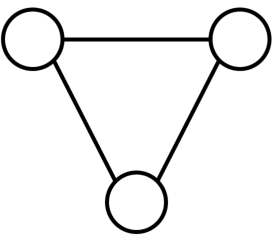
\includegraphics[scale=0.5]{graph-basic}
	\end{flushright}
	\vspace{0.1cm}
	\begin{tiny}
		\begin{columns}
			\column{.45\textwidth}
\begin{lstlisting}
public class Graph {
	List nodes = new ArrayList();
	List edges = new ArrayList();

	Edge add(Node n, Node m) {
		Edge e = new Edge(n, m);
		nodes.add(n); nodes.add(m); edges.add(e);
		return e;
	}
	void print() {
		for (int i = 0; i < edges.size(); i++) {
			((Edge) edges.get(i)).print();
		}
	}
}
\end{lstlisting}
			\column{.45\textwidth}
\begin{lstlisting}
public class Node {
	int id = 0;

	void print() {
		System.out.print(id);
	}
}
\end{lstlisting}
\begin{lstlisting}
public class Edge {
	Node a, b;

	Edge(Node _a, Node _b) {
		a = _a; b = _b;
	}
	void print() {
		a.print(); b.print();
	}
}
\end{lstlisting}
		\end{columns}
	\end{tiny}
\end{frame}

\begin{frame}[fragile]{Evolution Step: Weighted Graphs}
	\vspace{-1.5cm}
	\begin{flushright}
		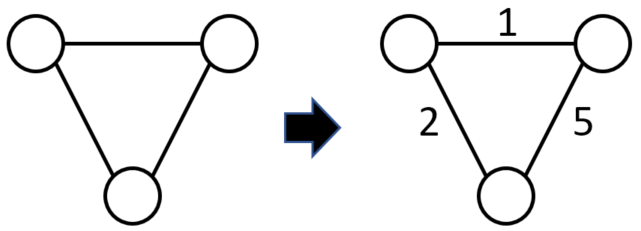
\includegraphics[scale=0.5]{graph-basic-to-weighted}
	\end{flushright}
	\vspace{0.1cm}
	\begin{tiny}
		\begin{columns}
			\column{.45\textwidth}
\begin{lstlisting}
public class Graph {
	List nodes = new ArrayList();
	List edges = new ArrayList();

	Edge add(Node n, Node m) {
		Edge e = new Edge(n, m);
		nodes.add(n); nodes.add(m); edges.add(e);
		@e.weight = new Weight();@
		return e;
	}
	@Edge add(Node n, Node m, Weight w) {
		Edge e = new Edge(n, m);
		nodes.add(n); nodes.add(m); edges.add(e);
		e.weight = w;
		return e;
	}@
	void print() {
		for (int i = 0; i < edges.size(); i++) {
			((Edge) edges.get(i)).print();
		}
	}
}
\end{lstlisting}
			\column{.45\textwidth}
\begin{lstlisting}
public class Edge {
	Node a, b;
	@Weight weight = new Weight();@

	Edge(Node _a, Node _b) {
		a = _a; b = _b;
	}
	void print() {
		a.print(); b.print();
		@weight.print();@
	}
}
\end{lstlisting}
\begin{lstlisting}
@public class Weight {
	void print() {...}
}@
\end{lstlisting}
		\end{columns}
	\end{tiny}
\end{frame}

\begin{frame}[fragile]{Evolution Step: Colored Graphs}
	\vspace{-1.5cm}
	\begin{flushright}
		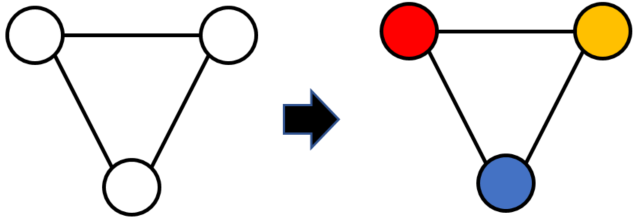
\includegraphics[scale=0.5]{graph-basic-to-colored}
	\end{flushright}
	\vspace{0.1cm}
	\begin{tiny}
		\begin{columns}
			\column{.45\textwidth}
\begin{lstlisting}
public class Graph {
	List nodes = new ArrayList();
	List edges = new ArrayList();

	Edge add(Node n, Node m) {
		Edge e = new Edge(n, m);
		nodes.add(n); nodes.add(m); edges.add(e);
		return e;
	}
	void print() {
		for (int i = 0; i < edges.size(); i++) {
			((Edge) edges.get(i)).print();
		}
	}
}
\end{lstlisting}	
			\column{.45\textwidth}
\begin{lstlisting}
public class Node {
	int id = 0;
	~Color color = new Color();~

	void print() {
		~Color.setDisplayColor(color);~
		System.out.print(id);
	}
}
\end{lstlisting}
\begin{lstlisting}
~public class Color {
	static void setDisplayColor(Color c) {...}
}~
\end{lstlisting}
		\end{columns}
	\end{tiny}
\end{frame}

\begin{frame}{Problem: Dealing With New Requirements}
	\leftorright{
		\myexample{New requirement}{
			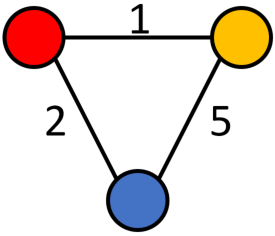
\includegraphics[scale=0.4]{graph-weighted-colored}
		}
	}{
		\myexample{Where to start from?}{
			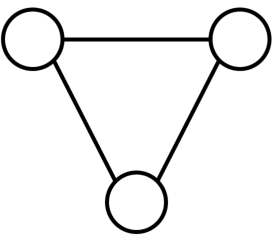
\includegraphics[scale=0.4]{graph-basic}
			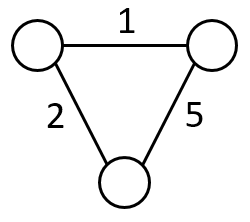
\includegraphics[scale=0.4]{graph-weighted}
			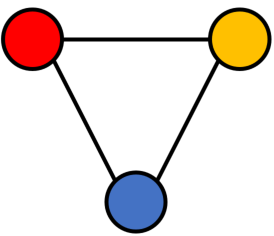
\includegraphics[scale=0.4]{graph-colored}
		}
	}
\end{frame}

\begin{frame}[fragile]{Problem: Evolution and Maintenance}
	\begin{columns}
		\column{.15\textwidth}
			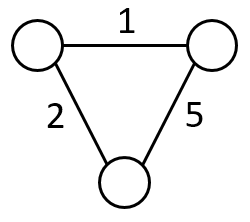
\includegraphics[width=\linewidth]{graph-weighted}
		\column{.3\textwidth}
\begin{tiny}
\begin{lstlisting}
public class Graph {
	...
	Edge add(Node n, Node m) {
		Edge e = new Edge(n, m);
		nodes.add(n); nodes.add(m); edges.add(e);
		@e.weight = new Weight();@
		return e;
	}
	@Edge add(Node n, Node m, Weight w) {
		Edge e = new Edge(n, m);
		nodes.add(n); nodes.add(m); edges.add(e);
		e.weight = w;
		return e;
	}@
	...
}
\end{lstlisting}
\end{tiny}
		\column{.025\textwidth}
			\begin{LARGE}
				$\Rightarrow$
			\end{LARGE}
		\column{.3\textwidth}
\begin{tiny}
\begin{lstlisting}
public class Graph {
	...
	Edge add(Node n, Node m) {
		Edge e = new Edge(n, m);
		nodes.add(n); nodes.add(m); edges.add(e);
		@e.weight = new Weight();@
		return e;
	}
	@Edge add(Node n, Node m, Weight w) {
		Edge e = this(n, m);
		e.weight = w;
		return e;
	}@
	...
}
\end{lstlisting}
\end{tiny}
	\end{columns}
	\myexample{Where and how to propagate the improvement (here: refactoring)}{
		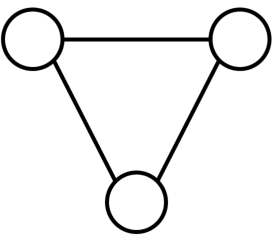
\includegraphics[scale=0.4]{graph-basic}
		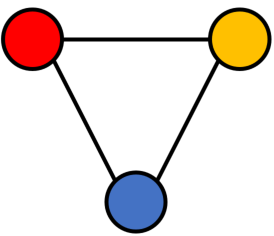
\includegraphics[scale=0.4]{graph-colored}
		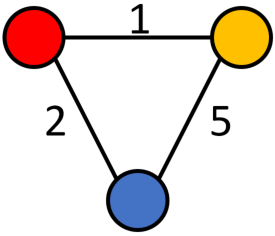
\includegraphics[scale=0.4]{graph-weighted-colored}
	}
\end{frame}

\lessonslearned{
	\item Compile-time variability is decided before or at compile time.
	\item In Clone-and-Own, new variants of a software system are created by copying and adapting an existing variant.
	\item Simple paradigm, but suffering from maintenance problems in the long run.
}{
	\item \todo{\ldots}
}{
	\begin{itemize}
		\item What are the reasons why clone-and-own is very popular in practice?
		\item What is the order of magnitude of the number of variants that can be reasonably maintained in clone-and-own?
		\item Have you ever applied the principle of clone-and-own? If so, where and how? 
	\end{itemize}
}

\sectionend

\section{Clone-and-Own with Version Control}


\subsection{Software Configuration Management}

\begin{frame}{Excursus: Software Configuration Management}
	\frameSoftwareConfigurationManagement
\end{frame}

\begin{frame}{Excursus: Software Configuration Management}
	\begin{mycolumns}[widths={45},animation=none]
		\begin{definition}{Basic Terms and Definitions} % TODO source missing
			\begin{itemize}
				\item {\bf Software Item}: An (atomic) artifact that can be uniquely identified
				\item {\bf Version}: A modified software item
				\begin{itemize}
					\item {\bf Revision}: A new version that replaces an old one
					\item {\bf Variant}: A version that co-exists with another one
				\end{itemize}
				\uncover<2->{
					\item {\bf Configuration}: A set of software items that together form a functioning (partial) system % TODO term is confusing and overloaded in next lecture + it appears to me that this was only needed in the good old days with CVS with versioning on a per file basis
					\item {\bf Baseline}: A stable configuration that represents a point of reference for further development
					\item {\bf Release}: A baseline delivered to customers
				}
			\end{itemize}
		\end{definition}
	\mynextcolumn
		\only<1|handout:0>{\pic[width=\linewidth]{configuration-management-1}}%
		\only<2-|handout:1>{\pic[width=\linewidth]{configuration-management-2}}%
	\end{mycolumns}	
\end{frame}

\begin{frame}{Example: A Conceptual Organization of our Graph Library}
	\centering
	\only<1|handout:0>{\pic[width=0.8\linewidth]{configuration-management-graphs-1}}%
	\only<2-|handout:1>{\pic[width=0.8\linewidth]{configuration-management-graphs-2}}%
\end{frame}
% TODO axis labels missing on this slide

%\begin{frame}{Tool Support: Version Control Systems}
	%\only<1|handout:0>{\pic[width=\linewidth,page=1]{branching}}%
	%\only<2|handout:0>{\pic[width=\linewidth,page=2]{branching}}%
	%\only<3-|handout:1>{\pic[width=\linewidth,page=3]{branching}}%
%\end{frame}

\subsection{Version Control Systems}

\begin{frame}{Tool Support: Version Control Systems}
	\centering
	\uncover<4->{\hspace{30mm}$\text{cherrypick := patch}(\Delta(r8,r10),r11)$}

	\vfill
	\only<1|handout:0>{\pic[width=0.6\linewidth]{versioncontrol-1}}%
	\only<2|handout:0>{\pic[width=0.6\linewidth]{versioncontrol-2}}%
	\only<3-|handout:1>{\pic[width=0.6\linewidth]{versioncontrol-3}}\\

	\vfill
	\uncover<5->{$\text{merge := 3-way-merge}(r4,\Delta(r4,r7),\Delta(r4,r9))$}
\end{frame}
% TODO no actual merges shown, only fast-forward
% TODO cherry pick needs to point to an arrow, not a node

\subsection{Supporting Clone-and-Own Development}

\begin{frame}{Example: Graph Library under Version Control}
	\centering\pic[width=0.7\linewidth]{versioncontrol-graphs-1}
\end{frame}

\begin{frame}{Example: Graph Library under Version Control}
	\centering\pic[width=0.7\linewidth]{versioncontrol-graphs-2}
\end{frame}

\begin{frame}{Example: Graph Library under Version Control}
	\centering\pic[width=0.7\linewidth]{versioncontrol-graphs-3}
\end{frame}

\subsection{Discussion}

\begin{frame}{Clone-and-Own with Version Control}
	\begin{mycolumns}[widths={60}]
		\begin{note}{Observations}
			\begin{itemize}
				\item aka.\ \emph{managed clone-and-own} (opposed to ad-hoc clone-and-own)
				\item Supports keeping tracking of revisions and variants\\-- aka.\ \emph{provenance} \deutsch{Herkunft}
				\item Creation of new variants is partially supported by merging of branches
				\item Propagation of changes between variants is supported by cherrypicking changes
			\end{itemize}
			However:
			\begin{itemize}
				\item Versioning is typically limited to entire system variants (i.e., branches)
				\item No flexible combination of software items
			\end{itemize}
		\end{note}
	\mynextcolumn
		\begin{note}{Advantages}
			\begin{itemize}
				\item Well-established and stable systems
				\item Well-known known process
				\item Good tool integration	
			\end{itemize}
		\end{note}
		\begin{note}{Disadvantages}
			\begin{itemize}
				\item Development of variants, not features: flexible combination of features not directly possible
				\item No structured reuse (copy \& edit)
				\item Merging and cherrypicking not fully automated
			\end{itemize}	
		\end{note}
	\end{mycolumns}
\end{frame}


\lessonslearned{
	\item Software Configuration Management as a traditional discipline of managing the evolution of variability-intensive systems 
	\item Version Control Systems as a widespread tool supporting Clone-and-Own in Practice
}{
	\item \fospl, Chapter 5.1
}{
	\begin{itemize}
		\item Which Software Configuration Management concepts are supported by Version Control Systems?
		\item Do you know other version control systems than Git? 
		\item If so, in which way are they different from Git? 
	\end{itemize}
}

\sectionend

\section{Clone-and-Own with Build Systems}


\begin{frame}{Recap: Software Configuration Management}
	\vspace{2mm}
	\pic[width=0.7\linewidth]{configuration-management-2}
\end{frame}

\subsection{Build Systems}

\begin{frame}{Tool Support: Build Systems}
	\begin{mycolumns}[columns=2,widths={50,50},animation=none]
		\pic[width=\linewidth]{ant-hello-world}		
	\mynextcolumn
		\mydefinition{Build Systems}{	
			\begin{itemize}
				\item Automation of the build process through build scripts
				\item Multiple steps with dependencies/conditions
				\begin{itemize}
					\item Copy files, 
					\item call compiler, 
					\item start other tools, 
					\item \ldots
				\end{itemize}	
				\item Tools: 
				\begin{itemize}
					\item make
					\item ant
					\item maven
					\ldots
				\end{itemize}
			\end{itemize}
		}
	\end{mycolumns}	
\end{frame}

\subsection{Variability through Build Scripts}

\begin{frame}{Variability through Build Scripts}
	\begin{flushright}		
		\vspace{-1cm}
		\pic[scale=0.27]{buildsystems}
		~~~~~~~~~~~~~~~~~
	\end{flushright}
	\begin{mycolumns}[columns=2,widths={50,50},animation=none]
		\vspace{-8cm}
		\mynote{Basic Idea}{	
			\begin{itemize}
				\item One build script per variant.
				\item Include/exclude files when translating.
				\item Overwrite variant-specific files.
			\end{itemize}
		}		
	\mynextcolumn
		~	
	\end{mycolumns}	
\end{frame}

\begin{frame}[fragile]{Example: Graph Library}
\begin{tiny}	
	\begin{mycolumns}[columns=4,widths={10,30,10,60},animation=none]
		~
	\mynextcolumn
		\vspace{2mm}
		\pic[width=\linewidth]{buildsystems-graphs-1}	% ist die fehlende Kante zu Graph beabsichtigt? das kann ja nicht klappen, oder?
	\mynextcolumn
		~
	\mynextcolumn
\begin{codetight}{}
public class Edge {
	Node a, b;

	Edge(Node _a, Node _b) {
		a = _a; b = _b;
	}
	...
}
\end{codetight}
\vspace{1cm}
\begin{codetight}{}
public class Edge {
	Node a, b;
	@Weight weight = new Weight();@

	Edge(Node _a, Node _b) {
		a = _a; b = _b;
	}
	...
}
\end{codetight}
	\end{mycolumns}
\end{tiny}
\end{frame}

\begin{frame}[fragile]{Example: Graph Library}
\begin{tiny}	
	\begin{mycolumns}[columns=4,widths={10,30,10,60},animation=none]
		~
	\mynextcolumn
		\vspace{2mm}
		\pic[width=\linewidth]{buildsystems-graphs-2}	
	\mynextcolumn
		~
	\mynextcolumn
\begin{codetight}{}
public class Graph implements IGraph {
	@EdgeFactory ef;@
	...
	@public Graph(EdgeFactory _ef) {
		ef = _ef;@
	}
	public Edge add(Node n, Node m) {
		@Edge e = ef.createEdge(n, m);@
		nodes.add(n); nodes.add(m); edges.add(e);
		return e;
	}
	...
}
\end{codetight}
\begin{codetight}{}
public class Edge {
	Node a, b;
	...
}
\end{codetight}
\vspace{0.5cm}
\begin{codetight}{}
public class WeightedEdge extends Edge {
	Node a, b;
	@Weight weight = new Weight();@
	...
}
\end{codetight}
	\end{mycolumns}
\end{tiny}
\end{frame}

\subsection{Discussion}

\begin{frame}{Discussion}
	\begin{flushright}		
		\vspace{-1cm}
		\pic[scale=0.27]{buildsystems}
		~~~~~~~~~~~~~~~~~
	\end{flushright}
	\begin{mycolumns}[columns=2,widths={50,50},animation=none]
		\vspace{-8cm}
		\mynote{Comparison to Version Control Systems}{	
			\begin{itemize}
				\item Supports combination of more fine-grained software items (i.e., files).
				\item However: No provenance support.
			\end{itemize}
		}	
		\mynote{More generally:}{	
			\begin{itemize}
				\item Combination of items (i.e., files) $\neq$ combination of features.
				\item All variants are potentially affected by changes to the basic variant.
			\end{itemize}
		}		
	\mynextcolumn
		~	
	\end{mycolumns}	
\end{frame}

\lessonslearned{
	\item Variability through build scripts
	\item Granularity of clones: Individual files
	\item Combination of files $\neq$ combination of features
}{
	\item \fospl, Chapter 5.1
}{
	\begin{itemize}
		\item Which software configuration management concepts are supported by build systems?
		\item What are the commonalities and differences of clone-and-own with version control and clone-and-own with build systems?
		\item What are the strengths and weaknesses?
	\end{itemize}
}

\sectionend

\begin{frame}{\inserttitle}
	\lectureseriesoverview[I]
\end{frame}

\mode<beamer>{
	\begin{frame}{\inserttitle}
		\lectureseriesoverview
	\end{frame}

	\contentoverview
}


\end{document}
